\section{Resultados e Discussão}
\label{sec:resultados}

A execução integral da abordagem metodológica sobre as bases consolidadas de Divinópolis/MG em 2025 demonstrou capacidade de compressão estrutural e separação entre riscos críticos, passivos inativos e falsos positivos onomásticos. Em observância ao protocolo ético e à LGPD, todos os atores privados e sócios são designados exclusivamente por seus pseudônimos oficiais.

\begin{figure*}[!t]
\centering
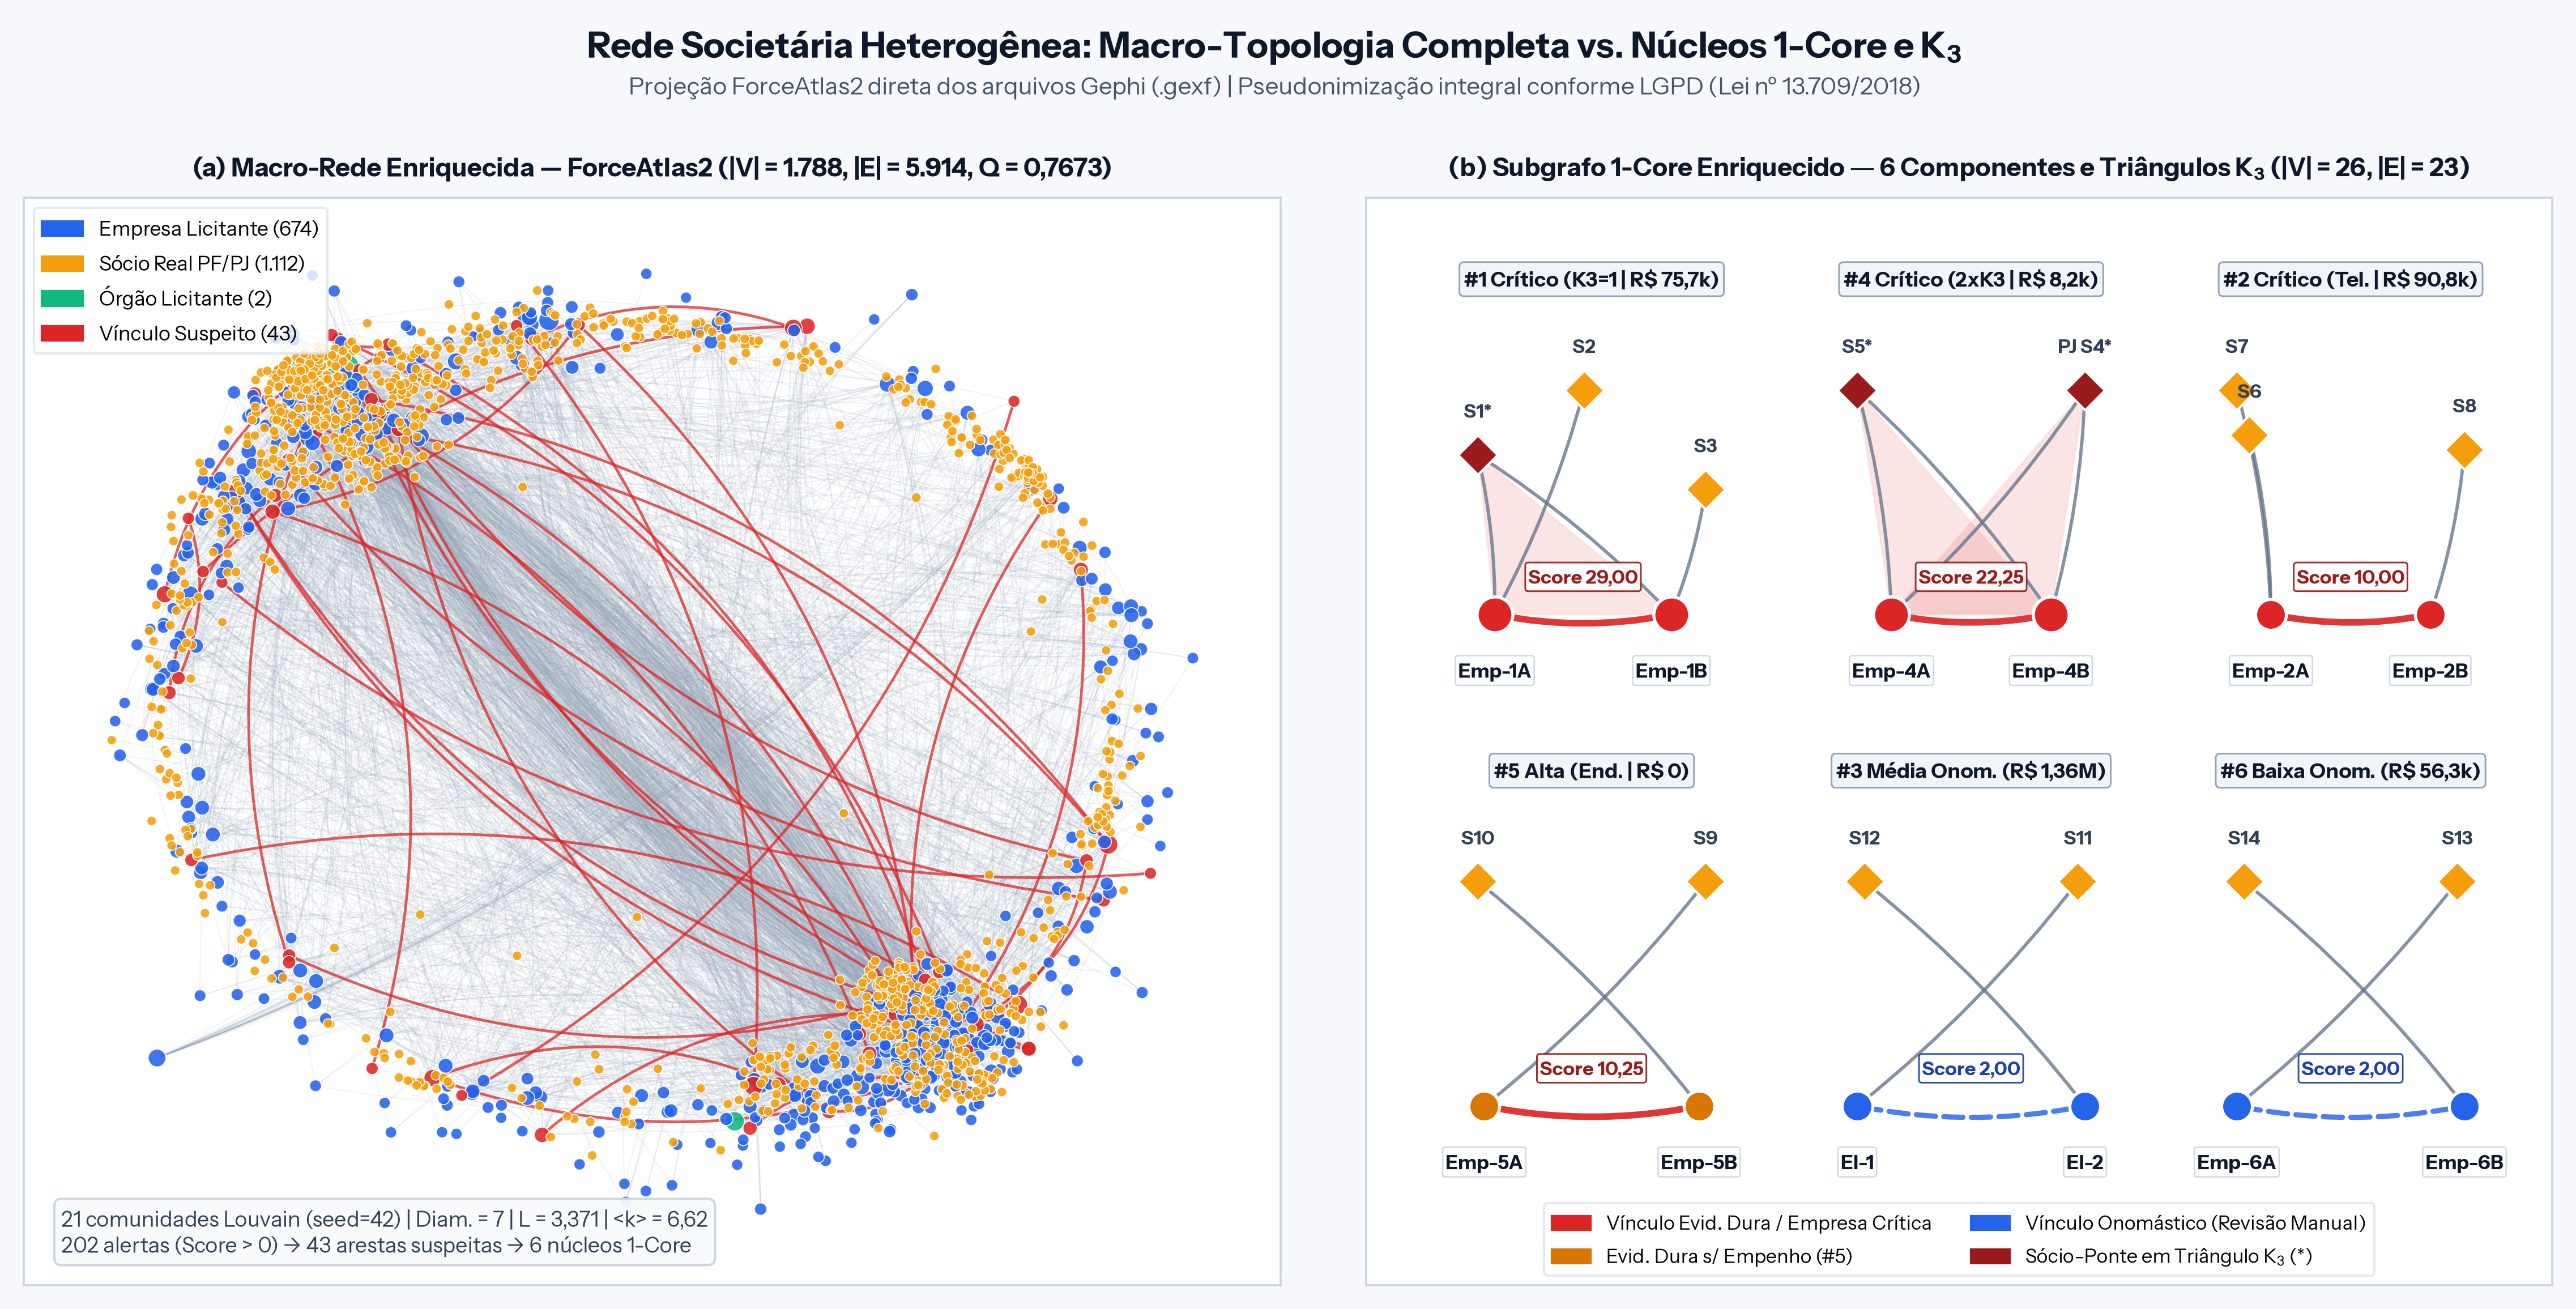
\includegraphics[width=0.72\textwidth]{figures/eixo1_rede_societaria_k3.png}
\caption{Visualização ForceAtlas2 dos grafos Gephi (\texttt{.gexf}) do módulo \texttt{01\_\allowbreak analise\_\allowbreak socios}: (a) macro-rede enriquecida (\texttt{grafo\_\allowbreak cheio.gexf}, $|V|=1.788$, $|E|=5.914$, $Q=0{,}7673$, 21 comunidades Louvain) destacando as 43 arestas \textnormal{\textit{Vinculo\_\allowbreak Suspeito}} (37 \texttt{MEDIO} e 6 \texttt{ALTO}, plotadas em vermelho no painel e diferenciadas entre âmbar e vermelho no \texttt{.gexf}); e (b) subgrafo $1$-core enriquecido (\texttt{subgrafos\_\allowbreak fraudes\_\allowbreak enriquecido.gexf}, $|V|=26$, $|E|=23$) exibindo os 6 componentes e triângulos $K_3$ sombreados (\#1 e \#4).}
\label{fig:eixo1_rede}
\end{figure*}

\subsection{Evolução Estrutural ao Longo das Quatro Etapas}

Na Etapa~1 (\texttt{01\_\allowbreak limpeza\_\allowbreak dados.py}), o saneamento documental produziu um grafo base de \textbf{2.589 vértices} (2 órgãos licitantes — Executivo \texttt{Orgao\_02} e Legislativo \texttt{Orgao\_01} —, 674 empresas licitantes e 1.913 registros provisórios \texttt{seq\_\allowbreak quadro\_\allowbreak soc}) e \textbf{6.652 arestas} (4.059 de \textit{Concorreu\_\allowbreak Contra}, 1.913 de \textit{É\_\allowbreak Dono\_\allowbreak De} e 680 de \textit{Participou\_\allowbreak Licitacao}). Dos 674 documentos licitantes, 673 correspondiam a CNPJs válidos de 14 dígitos e 1 constituía registro mascarado na base pública, cuja participação representou 13 arestas no grafo cheio (12 de \textit{Concorreu\_\allowbreak Contra} e 1 de \textit{Participou\_\allowbreak Licitacao}), 0 itens homologados e 2 empenhos somando R\$\,4.620,00 líquidos (R\$\,0,00 pagos).

Na Etapa~2 (\texttt{02\_\allowbreak enriquecimento\_\allowbreak socios.py}), a resolução cadastral via BrasilAPI atingiu \textbf{100,0\% de cobertura sobre os 673 CNPJs válidos} (\textbf{620} com QSA da Receita Federal e \textbf{53} titulares MEI/EI extraídos da razão social, zero vazios ou erros), recuperando \textbf{1.132 vínculos societários válidos} (1.079 QSA + 53 MEI/EI) e consolidando homônimos sequenciais em \textbf{1.112 vértices \textit{Sócio Real}} únicos. Substituindo os nós provisórios e incorporando as 43 arestas suspeitas paralelas (37 de nível \texttt{MEDIO} e 6 de nível \texttt{ALTO}), o grafo cheio (\texttt{grafo\_\allowbreak cheio.gexf}) alcançou \textbf{1.788 vértices} e \textbf{5.914 arestas}, formando uma única componente conexa ($\text{WCC}=1$, diâmetro 7, distância geodésica média $L=3{,}371$) organizada no multigrafo em 21 comunidades de Louvain (\texttt{seed=42}) com elevada modularidade ($Q=0{,}7673$).

O cômputo de escores sobre os 4.059 pares co-disputantes gerou exatamente \textbf{202 alertas com $\text{Score} > 0$}, cuja distribuição empírica consta na Figura~\ref{fig:eixo1_metricas}~(a). Verifica-se que \textbf{159 pares (78,7\%)} enquadram-se no nível \texttt{BAIXO} ($\text{Score}=0{,}25$ em 156 casos e $0{,}50$ em 3 casos, decorrentes de um ou dois sobrenomes frequentes) e \textbf{37 pares (18,3\%)} compõem o nível \texttt{MEDIO} ($\text{Score}=1{,}00$ em 34 casos e $1{,}25$ em 3 casos). Segundo \texttt{resumo\_\allowbreak auditoria\_\allowbreak eixo1\allowbreak .json}, esse estrato \texttt{MEDIO} podado pelo corte $w \ge 2{,}0$ envolve \textbf{61 empresas distintas} (30 pares com empenho bilateral, 4 com unilateral e 3 sem empenho), acumulando \textbf{R\$\,11.342.332,96} em soma par a par ou \textbf{R\$\,9.114.055,59} líquidos em empresas distintas (R\$\,444.663,53 homologados e R\$\,6.474.916,37 pagos), preservado em \texttt{alertas\_\allowbreak vinculos\_\allowbreak concorrentes\allowbreak .csv} sem contaminar o subgrafo crítico. Apenas \textbf{6 pares (3,0\%)} atingiram o limiar de alto risco ($\text{Score} \ge 2{,}0$), concentrando integralmente as coincidências objetivas detectadas no município: 2 pares com sócios em comum, 2 com mesmo endereço comercial, 2 com mesmo telefone corporativo, nenhum par com e-mail compartilhado (após filtragem de escritórios contábeis) e nenhum par com mesma raiz de CNPJ.

Na Etapa~3 (\texttt{03\_\allowbreak reduzir\_\allowbreak grafo.py}), a cadeia determinística de indução ($w \ge 2{,}0$, descartando as 37 arestas \texttt{MEDIO} e retendo apenas as 6 arestas \texttt{ALTO}), poda $1$-core via BFS e Union-Find comprimiu os 1.788 vértices da macro-rede para apenas \textbf{26 vértices} (12 empresas e 14 sócios) e \textbf{23 arestas} (6 arestas \textit{Vinculo\_\allowbreak Suspeito} e 17 arestas \textit{É\_\allowbreak Dono\_\allowbreak De}), reduzindo em \textbf{98,5\%} a cardinalidade de vértices auditados. Esse corte isolou \textbf{6 componentes conexos} independentes e enumerou \textbf{3 triângulos societários fechados ($K_3$)}, conforme ilustrado na projeção \textit{ForceAtlas2} da Figura~\ref{fig:eixo1_rede}.

\subsection{Anatomia dos Seis Componentes, Triângulos $K_3$ e Materialidade}

Na Etapa~4 (\texttt{04\_\allowbreak materialidade\_\allowbreak financeira.py}), o cruzamento por CNPJ/CPF higienizado abrangeu todas as 674 empresas do grafo base: apenas 88 apresentaram valor homologado positivo em \texttt{homolog\allowbreak Licitacao\allowbreak .csv} (somando R\$\,25.771.978,02 em 929 itens homologados), ao passo que \textbf{527 empresas} registraram empenhos contratuais líquidos positivos em 2025 (totalizando \textbf{R\$\,140.293.315,49}, dos quais R\$\,70.440.903,07 foram pagos a 454 credores). A Figura~\ref{fig:eixo1_componentes} expõe a topologia individual dos seis núcleos reduzidos, enquanto a Tabela~\ref{tab:eixo1_ranking} apresenta o \textit{ranking} completo de priorização.

\begin{figure*}[!t]
\centering
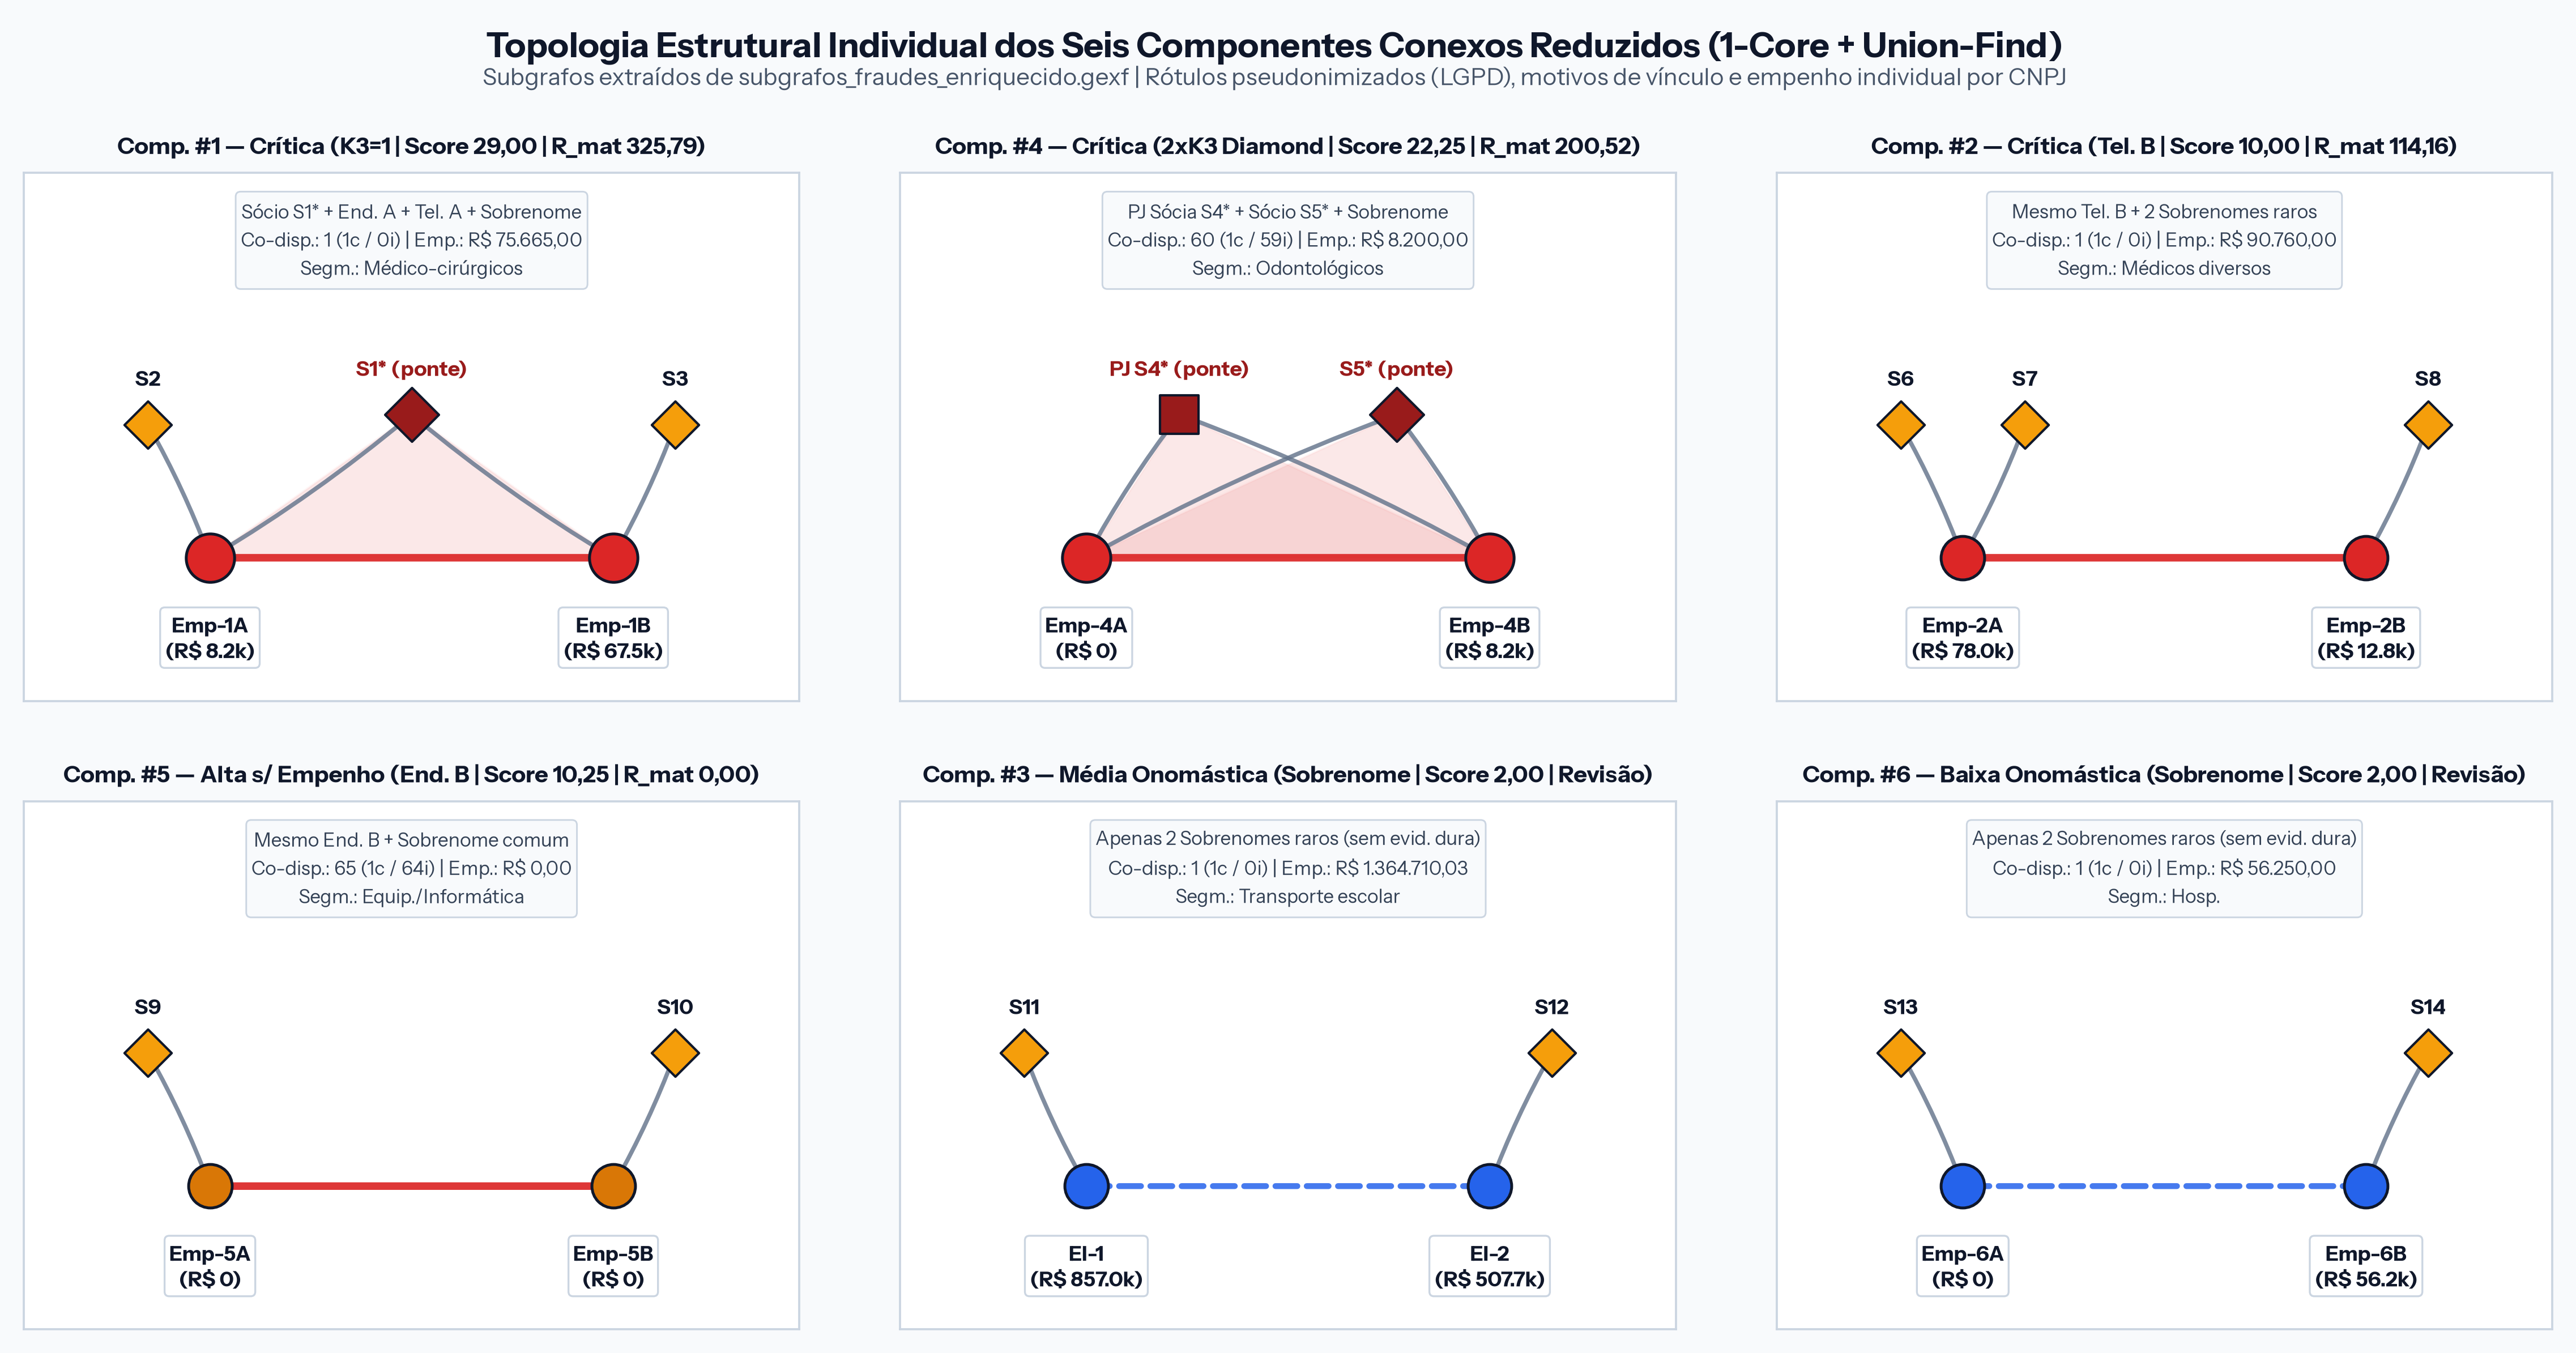
\includegraphics[width=0.71\textwidth]{figures/eixo1_componentes_detalhados.png}
\caption{Inspeção estrutural individual dos seis componentes conexos em \texttt{subgrafos\_\allowbreak fraudes\_\allowbreak enriquecido.gexf}, detalhando os triângulos $K_3$ simples (\#1) e duplo/diamante $K_4-e$ (\#4), cadeias acíclicas por telefone/endereço (\#2 e \#5), falsos positivos onomásticos (\#3 e \#6), decomposição de co-disputas (\textit{certames/itens}), segmento de objeto e empenho líquido por CNPJ sob pseudonimização LGPD.}
\label{fig:eixo1_componentes}
\end{figure*}

\begin{table*}[!t]
\centering
\caption{Ranking de priorização dos seis componentes conexos após cruzamento financeiro e filtro anti-falso positivo.}
\label{tab:eixo1_ranking}
\resizebox{\textwidth}{!}{%
\begin{tabular}{@{}clccllrrrrl@{}}
\toprule
\textbf{Comp.} & \textbf{Par Concorrente} & \textbf{Cert. / Itens} & \textbf{Score} & \textbf{Segmento} & \textbf{Critérios / Padrão Topológico} & \textbf{Empenhado Líq.} & \textbf{Pago Líq.} & \textbf{Risco Mat.} & \textbf{Classificação Final} \\
\midrule
\#1 & \texttt{Emp-1A} $\times$ \texttt{Emp-1B} & 1c / 0i & 29,00 & Médico-cirúrgicos & \texttt{S1*}, \texttt{End. A}, \texttt{Tel. A} ($K_3=1$) & R\$\,75.665,00 & R\$\,64.120,00 & 325,79 & Crítica (Evid. Dura + Contrato) \\
\#4 & \texttt{Emp-4A} $\times$ \texttt{Emp-4B} & 1c / 59i & 22,25 & Odontológicos & \texttt{PJ S4*}, \texttt{S5*} ($2\times K_3$, $K_4-e$) & R\$\,8.200,00 & R\$\,8.200,00 & 200,52 & Crítica (Evid. Dura + Contrato) \\
\#2 & \texttt{Emp-2A} $\times$ \texttt{Emp-2B} & 1c / 0i & 10,00 & Médicos diversos & \texttt{Tel. B}, 2 sobr. raros (árvore) & R\$\,90.760,00 & R\$\,87.200,00 & 114,16 & Crítica (Evid. Dura + Contrato) \\
\#5 & \texttt{Emp-5A} $\times$ \texttt{Emp-5B} & 1c / 64i & 10,25 & Equip./Informática & \texttt{End. B}, sobr. comum ($P_4$) & R\$\,0,00 & R\$\,0,00 & 0,00 & Alta (Evid. Dura s/ Empenho) \\
\#3 & \texttt{EI-1} $\times$ \texttt{EI-2} & 1c / 0i & 2,00 & Transporte escolar & Apenas 2 sobr. raros ($P_4$) & R\$\,1.364.710,03 & R\$\,819.965,10 & 28,25 & Média Onomástica (Rev. Manual) \\
\#6 & \texttt{Emp-6A} $\times$ \texttt{Emp-6B} & 1c / 0i & 2,00 & Hosp. & Apenas 2 sobr. raros ($P_4$) & R\$\,56.250,00 & R\$\,44.550,00 & 21,88 & Baixa Onomástica (Rev. Manual) \\
\bottomrule
\end{tabular}%
}
\end{table*}

Uma discussão crítica dos números da Tabela~\ref{tab:eixo1_ranking} revela dois aspectos metodológicos essenciais que explicam o comportamento do modelo:
\begin{enumerate}
  \item \textbf{Divergência entre homologações e empenhos} (\texttt{Vlr\_\allowbreak Homologado} nulo): nos seis componentes reduzidos, nenhuma das 12 empresas figurou como vencedora nos 929 registros de \texttt{homolog\allowbreak Licitacao\allowbreak .csv} de 2025, embora 5 componentes tenham movimentado empenhos contratuais expressivos. Esse fenômeno decorre do fato de que \texttt{homolog\allowbreak Licitacao\allowbreak .csv} cobre apenas 88 vencedores no exercício, deixando de fora empenhos oriundos de licitações homologadas em anos anteriores com execução continuada em 2025, adesões a atas e contratações diretas/dispensas não registradas na homologação licitatória. Caso a Etapa~4 dependesse exclusivamente das homologações do ano, todos os seis núcleos teriam materialidade nula; a regra de prioridade para \texttt{Vlr\_\allowbreak Empenhado\_\allowbreak Liq} garante cobertura efetiva da despesa contratada;
  \item \textbf{Rebaixamento consistente do Componente \#3 sem contradição:} embora o par \texttt{EI-1} $\times$ \texttt{EI-2} some R\$\,1.364.710,03 em 28 empenhos (\texttt{EI-1}: R\$\,856.966,20; \texttt{EI-2}: R\$\,507.743,83) e tenha atingido $\text{Score}=2{,}00$ pela coincidência de dois sobrenomes raros, o par não apresenta sócio em comum, mesma raiz CNPJ, endereço ou telefone (\texttt{Tem\_\allowbreak Evidencia\_\allowbreak Dura = False}). Em consonância com os Acórdãos do TCU~\cite{tcu2011acordao2341,tcu2024acordao1798}, a coincidência onomástica isolada — amplificada em bases de MEI/EI nas quais a Receita Federal não divulga o CPF do titular — não autoriza presunção de grupo econômico. O filtro da Etapa~4 preserva a rastreabilidade financeira (\texttt{MEDIA\_\allowbreak ONOMASTICA\_\allowbreak ALTA\_\allowbreak MATERIALIDADE} com \texttt{Validacao\_\allowbreak Manual = True}), posicionando \#3 ($R_{\text{mat}}=28{,}25$) abaixo dos três núcleos com evidência objetiva confirmada.
\end{enumerate}

\begin{table*}[!t]
\centering
\caption{Comparação topológica direta dos artefatos GEXF exportados para o Gephi no módulo \textnormal{\texttt{01\_\allowbreak analise\_\allowbreak socios}}.}
\label{tab:eixo1_gephi}
\resizebox{\textwidth}{!}{%
\begin{tabular}{@{}llrrrrrrrrr@{}}
\toprule
\textbf{Artefato (\texttt{.gexf})} & \textbf{Tipo} & \textbf{$|V|$} & \textbf{$|E|$} & \textbf{Densidade} & \textbf{$\langle k \rangle$} & \textbf{$\langle k_w \rangle$} & \textbf{$k_{\max}$} & \textbf{WCC (LCC)} & \textbf{$Q$ (Com. Louvain)} & \textbf{Diam. / $L$ (LCC)} \\
\midrule
\texttt{grafo\_cheio.gexf} (Etapa~2) & MultiGraph & 1.788 & 5.914 & 0,00370 & 6,62 & 80,06 & 628 & 1 (1.788) & 0,7673 (21) & 7 / 3,371 \\
\texttt{subgrafos\_fraudes.gexf} (Etapa~3) & Graph & 26 & 23 & 0,07077 & 1,77 & 7,12 & 3 & 6 (5) & 0,7512 (6) & 3 / 1,600 \\
\texttt{subgrafos\_fraudes\_enriquecido.gexf} (Etapa~4) & Graph & 26 & 23 & 0,07077 & 1,77 & 7,12 & 3 & 6 (5) & 0,7512 (6) & 3 / 1,600 \\
\bottomrule
\end{tabular}%
}
\par\vspace{2pt}{\footnotesize Notas: densidade e partição de Louvain (\texttt{seed=42}) computadas diretamente sobre o objeto NetworkX de cada \texttt{.gexf}; diâmetro e distância média $L$ avaliados na maior componente simples (LCC — nos subgrafos reduzidos, refere-se ao \texttt{Comp.~\#1} de 5 vértices; \texttt{Comp.~\#2}, também com 5 vértices, apresenta $L=1{,}800$, e a média global nos 44 pares conectados é $1{,}614$); $\langle k_w \rangle$ indica o grau médio ponderado.}
\end{table*}

\begin{figure*}[!t]
\centering
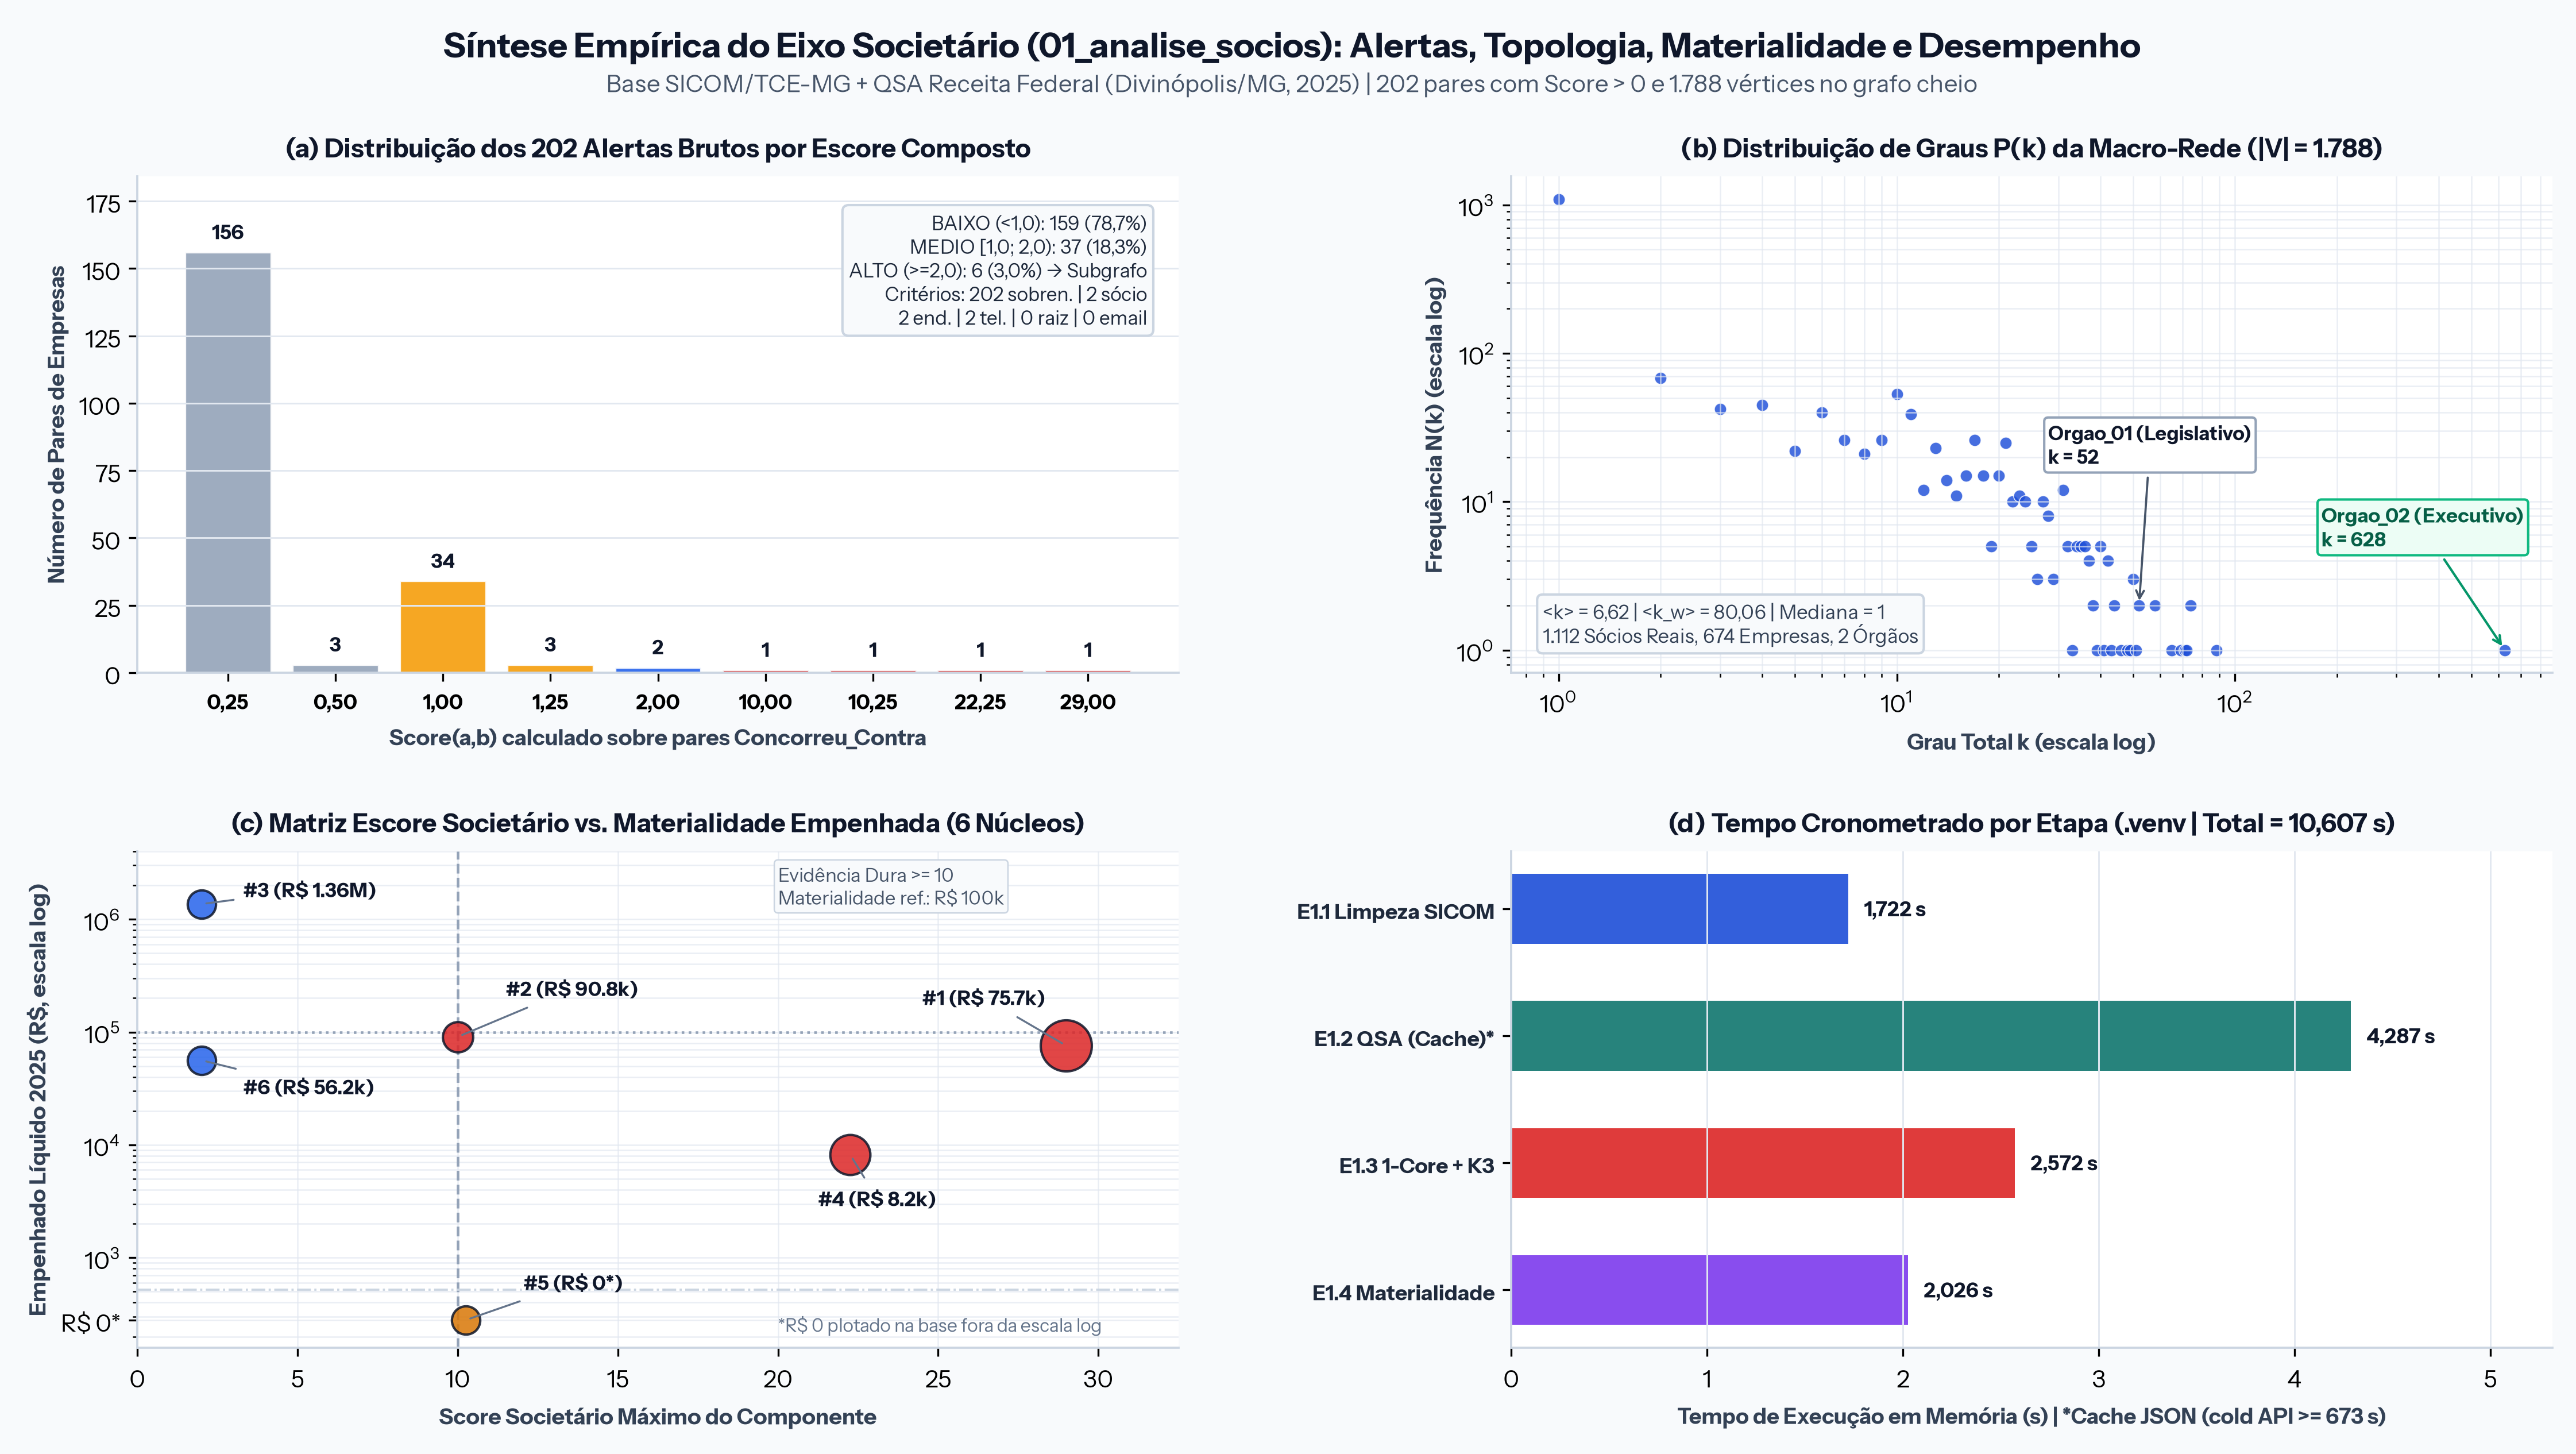
\includegraphics[width=0.71\textwidth]{figures/eixo1_metricas_topologicas.png}
\caption{Painel empírico de síntese do módulo \texttt{01\_\allowbreak analise\_\allowbreak socios}: (a) distribuição dos 202 alertas brutos por escore composto e estratificação \texttt{BAIXO}/\texttt{MEDIO}/\texttt{ALTO}; (b) distribuição de graus $P(k)$ em escala logarítmica da macro-rede ($|V|=1.788$) destacando \texttt{Orgao\_02} e \texttt{Orgao\_01}; (c) matriz \textit{Score} $\times$ Empenhado Líquido separando os núcleos críticos do falso positivo onomástico \#3; e (d) tempos cronometrados das quatro etapas em memória (10,607\,s).}
\label{fig:eixo1_metricas}
\end{figure*}

A inspeção dos seis núcleos agrupados por perfil estrutural na Figura~\ref{fig:eixo1_componentes} evidencia também a distinção comportamental revelada por \texttt{Cert.~/~Itens} e \texttt{Segmento\_\allowbreak Objeto}:
\begin{itemize}
  \item \textbf{Núcleo crítico \#1 ($K_3=1$, $R_{\text{mat}}=325{,}79$, Médico-cirúrgicos):} subgrafo de 5 vértices e 5 arestas conectando \texttt{Emp-1A} e \texttt{Emp-1B} pelo sócio-ponte \texttt{S1*} (fechando um triângulo $K_3$), mesmo endereço (\texttt{End.~A}) e mesmo telefone (\texttt{Tel.~A}, $\text{Score}=29{,}00$), com faturamento ativo em ambas (\texttt{Emp-1A}: R\$\,8.165,00; \texttt{Emp-1B}: R\$\,67.500,00) e atuação no mesmo certame sem sobreposição direta de itens no julgamento (\texttt{1c / 0i});
  \item \textbf{Núcleo crítico \#4 ($2\times K_3$, diamante $K_4-e$, $R_{\text{mat}}=200{,}52$, Odontológicos):} 4 vértices e 5 arestas em que tanto a pessoa jurídica sócia \texttt{PJ S4*} quanto \texttt{S5*} integram simultaneamente o QSA de \texttt{Emp-4A} e \texttt{Emp-4B} ($\text{Score}=22{,}25$). A decomposição \texttt{1c / 59i} confirma competição concentrada item a item em um único pregão (\textbf{60 co-disputas}) com assimetria financeira (\texttt{Emp-4A}: R\$\,0,00; \texttt{Emp-4B}: R\$\,8.200,00 pagos), padrão compatível com \textit{cover bidding} a ser auditado nas atas;
  \item \textbf{Núcleos cadastrais \#2 e \#5 ($\text{Tel.~B}$ e $\text{End.~B}$):} em \#2 (Médicos diversos, \texttt{1c / 0i}), sócios formalmente distintos (\texttt{S6}/\texttt{S7} e \texttt{S8}) compartilham telefone (\texttt{Tel.~B}) e dois sobrenomes raros ($\text{Score}=10{,}00$), somando R\$\,90.760,00 empenhados (R\$\,78.000,00 e R\$\,12.760,00); já \#5 (Equip./Informática, \texttt{1c / 64i}) apresenta padrão compatível com \textit{cover bidding} item a item no mesmo endereço (\texttt{End.~B}, \textbf{65 co-disputas}, $\text{Score}=10{,}25$), porém sem empenho em 2025 ($R_{\text{mat}}=0{,}00$);
  \item \textbf{Triagem onomástica \#3 e \#6 ($P_4$, $\text{Score}=2{,}00$, \texttt{1c / 0i}):} caminhos simples de 4 vértices em Transporte escolar (\#3) e Equipamentos hospitalares (\#6, R\$\,56.250,00 em \texttt{Emp-6B} e R\$\,0,00 em \texttt{Emp-6A}), ligados apenas por dois sobrenomes raros em itens distintos do mesmo certame para revisão manual de homonímia ou parentesco.
\end{itemize}

\subsection{Métricas Gephi, Topologia em Estrela e Desempenho Real}

A Tabela~\ref{tab:eixo1_gephi} compara as métricas topológicas extraídas diretamente dos três arquivos \texttt{.gexf} exportados para o Gephi. Entre a macro-rede (\texttt{grafo\_\allowbreak cheio.gexf}) e os subgrafos reduzidos (\texttt{subgrafos\_\allowbreak fraudes.gexf} e \texttt{subgrafos\_\allowbreak fraudes\_\allowbreak enriquecido.gexf}), a densidade cresce mais de 19 vezes ($0{,}00370 \to 0{,}07077$), o diâmetro da maior componente cai de 7 para 3 e a distância geodésica média reduz-se de $3{,}371$ para $1{,}600$ (\texttt{Comp.~\#1}), mantendo modularidade alta ($Q=0{,}7512$) exatamente alinhada aos 6 componentes de Union-Find. Os valores estruturais de \texttt{subgrafos\_\allowbreak fraudes.gexf} e \texttt{subgrafos\_\allowbreak fraudes\_\allowbreak enriquecido.gexf} coincidem porque a Etapa~4 agrega atributos financeiros e filtros sem alterar a topologia $|V|=26, |E|=23$.

\begin{table}[!t]
\centering
\caption{Tempos reais cronometrados por etapa de \textnormal{\texttt{01\_\allowbreak analise\_\allowbreak socios}} (cache local de 673 CNPJs).}
\label{tab:eixo1_benchmark}
\resizebox{\columnwidth}{!}{%
\begin{tabular}{@{}llcr@{}}
\toprule
\textbf{Etapa / Script} & \textbf{Volume Processado} & \textbf{Complexidade} & \textbf{Tempo (s)} \\
\midrule
E1.1 \texttt{01\_limpeza\_dados.py} & 4 CSVs $\to$ 2.589 nós / 6.652 ar. & $\mathcal{O}(N)$ & 1,722 \\
E1.2 \texttt{02\_enriquecimento\_socios.py} & 673/673 CNPJs (\textit{cache}) $\to$ 1.788 nós / 5.914 ar. & $\mathcal{O}(|E_{\text{conc}}|)$ & 4,287* \\
E1.3 \texttt{03\_reduzir\_grafo.py} & Indução, $1$-Core, Union-Find, $K_3$ $\to$ 26 nós & $\mathcal{O}(|V|+|E|\,d_{\max})$ & 2,572 \\
E1.4 \texttt{04\_materialidade\_financeira.py} & 674 empresas cruzadas + JSON/LGPD & $\mathcal{O}(N)$ & 2,026 \\
\midrule
\textbf{Total em Memória} & \textbf{Pipeline completo (4 etapas)} & -- & \textbf{10,607} \\
\bottomrule
\end{tabular}%
}
\par\vspace{2pt}{\footnotesize *Em execução fria sem \textit{cache}, a BrasilAPI impõe intervalo mínimo $\ge 1{,}0$\,s/CNPJ ($\ge 673$\,s $\approx$ 11,2\,min, $>98{,}4\%$ da latência total).}
\end{table}

Na distribuição de graus da macro-rede (Figura~\ref{fig:eixo1_metricas}b), destaca-se forte assimetria de cauda pesada: enquanto a mediana global vale $k=1$ (sócios vinculados a uma única sociedade), o grau médio é $\langle k \rangle = 6{,}62$ e os dois maiores concentradores pertencem aos órgãos licitantes (\texttt{Orgao\_02} com $k=628$ e força ponderada $k_w=836$; \texttt{Orgao\_01} com $k=52$ e $k_w=53$). Essa topologia gravitacional em estrela comprova a necessidade algorítmica da etapa de indução: se as arestas \textit{Participou\_\allowbreak Licitacao} não fossem removidas antes do Union-Find, os órgãos públicos manteriam praticamente todo o mercado colapsado em uma única componente gigante.

Por fim, a Tabela~\ref{tab:eixo1_benchmark} e a Figura~\ref{fig:eixo1_metricas}~(d) reportam os tempos reais cronometrados em Python (\texttt{-{}-offline} com \textit{cache} JSON): todo o \textit{pipeline} do módulo \texttt{01\_\allowbreak analise\_\allowbreak socios} executou ponta a ponta em \textbf{10,607\,s} (soma exata das quatro etapas), confirmando o comportamento linear e quase linear esperado mesmo após a extração setorial e o cruzamento completo de auditoria. O único gargalo significativo reside na coleta inicial de rede junto à BrasilAPI, que impõe ao menos 673\,s (11\,min\,13\,s) para os 673 CNPJs válidos devido ao limite de 1 requisição/segundo — tornando o \textit{cache} incremental em disco essencial para auditoria interativa e escalabilidade operacional.
